\appendix
\chapter{Tesztesetek}

\begin{figure}[H]
\begin{center}
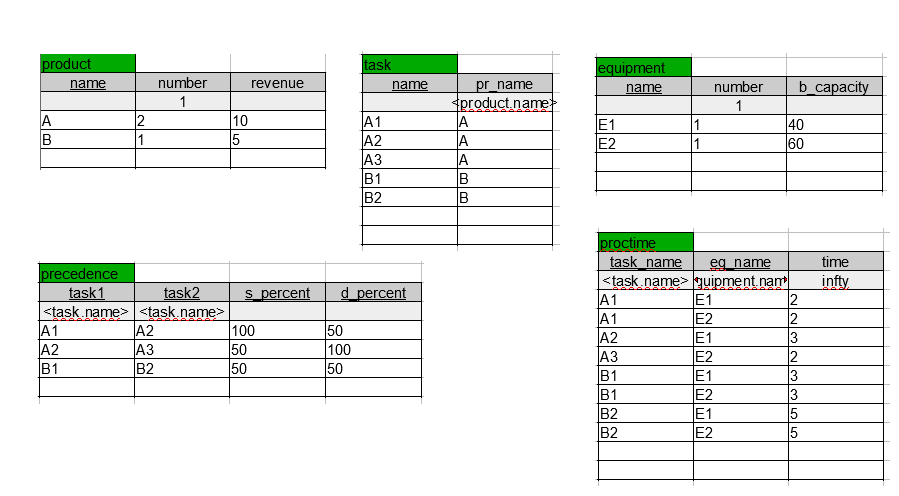
\includegraphics[scale=0.85]{teszteset8}
\caption{Nyolcadik teszteset bemeneti adatai}
\label{teszteset8}
\end{center}
\end{figure}

\begin{table}
	\begin{center}
	\caption{Második példafeladat teszteseteinek második fele}
  	\captionsetup[table]{skip=10pt}
  	\label{tab:table3}  	
  	\begin{sideways}  	  	
  		\begin{tabular}{|c|c|c|c|c|c|c|c|c|}
  		\hline
		Fájl név & Idő horizont & A termék & B termék & Kapacitások & Hozzárendelések & Bevétel & Megoldás ideje & Gantt \\
		\hline
		teszt06 & 25 & 2 db & 1 db & \makecell{A1: 100 \\ A1\_2: 100\\A2: 40\\A2\_2: 40\\A3: 40\\A3\_2:40\\B1: 100\\B2: 100} & \makecell{E1: A1, A1\_2,\\A2, A2\_2 \\B1, B2 \\E2: A1, A1\_2,\\ A3, A3\_2, \\ B1, B2} & 1300 & 0,162 sec & er06 \\
		\hline	
		teszt07 & 20 & 2 db & 1 db & \makecell{A1: 60\\A1\_2: 100\\A2: 40\\A2\_2: 40\\A3: 20\\A3\_2:20\\B1: 60\\B2: 60} & \makecell{E1: A1\_2, A2,\\A2\_2 \\ E2: A1, A1\_2,\\ A3, A3\_2, \\ B1, B2} & 700 & 0,844 sec & er07 \\
		\hline	
		teszt08 & 25 & 2 db & 1 db & \makecell{A1: 100 \\ A1\_2: 100\\A2: 40\\A2\_2: 40\\A3: 20\\A3\_2:20\\B1: 100\\B2: 100} & \makecell{E1: A1, A1\_2,\\A2, A2\_2 \\B1, B2 \\E2: A1, A1\_2,\\ A3, A3\_2, \\ B1, B2} & 900 & 0,220 sec & er08 \\
		\hline	
		\end{tabular}
	\end{sideways}
	\end{center}
\end{table}